\documentclass[12pt]{article}

\usepackage{amsmath,amsthm,amsfonts,amssymb,amsxtra}
\usepackage{pgf,tikz}
\usetikzlibrary{arrows}
\renewcommand{\theenumi}{(\alph{enumi})} 
\renewcommand{\labelenumi}{\theenumi}

\pagestyle{empty}
\setlength{\textwidth}{7in}
\setlength{\oddsidemargin}{-0.5in}
\setlength{\topmargin}{-1.0in}
\setlength{\textheight}{9.5in}

\theoremstyle{definition}
\newtheorem{problem}{Problem}

\newcommand{\sectionlinetwo}[2]{%
  \nointerlineskip \vspace{.5\baselineskip}\hspace{\fill}
  {\color{#1}
    \resizebox{0.5\linewidth}{2ex}
    {{%
    {\begin{tikzpicture}
    \node  (C) at (0,0) {};
    \node (D) at (9,0) {};
    \path (C) to [ornament=#2] (D);
    \end{tikzpicture}}}}}%
    \hspace{\fill}
    \par\nointerlineskip \vspace{.5\baselineskip}
  }

\makeatletter
\newcommand*{\radiobutton}{%
  \@ifstar{\@radiobutton0}{\@radiobutton1}%
}
\newcommand*{\@radiobutton}[1]{%
  \begin{tikzpicture}
    \pgfmathsetlengthmacro\radius{height("X")/2}
    \draw[radius=\radius] circle;
    \ifcase#1 \fill[radius=.6*\radius] circle;\fi
  \end{tikzpicture}%
}
\makeatother

\begin{document}

\noindent{\large\bf MATH 122}\hfill{\large\bf Exam \#2.}\hfill{\large\bf
  Fall 2016}\hfill{\large\bf Page 1/4}\hrule

\bigskip
\begin{center}
  \begin{tabular}{|ll|}
    \hline & \cr
    {\bf Name: } & \makebox[12cm]{\hrulefill}\cr & \cr
    {\bf VIP ID:} & \makebox[12cm]{\hrulefill}\cr & \cr
    \hline
  \end{tabular}
\end{center}
\begin{itemize}
\item Write your name and VIP ID in the space provided above.
\item The test has four (4) pages, including this one.
\item Enter your answer in the box(es) provided.
\item You must show sufficient work to justify all answers unless
  otherwise stated in the problem.  Correct answers with inconsistent
  work may not be given credit.
\item Credit for each problem is given in parentheses at the right of
  the problem number.
\item No books or notes may be used on this test.
\item An approved calculator may be used on this test.
\end{itemize}
\hrule
\vspace{2cm}

\begin{center}
  \begin{tabular}{|c|c|c|}
    \hline
    &&\cr
    {\large\bf Page} & {\large\bf Max.~points} & {\large\bf Your points} \cr
    &&\cr
    \hline
    &&\cr
    {\Large 2} & \Large 30 & \cr
    &&\cr
    \hline
    &&\cr
    {\Large 3} & \Large 49 & \cr
    &&\cr
    \hline
    &&\cr
    {\Large 4} & \Large 21 & \cr
    &&\cr
    \hline\hline
    &&\cr
    {\large\bf Total} & \Large 100 & \cr
    &&\cr
    \hline
  \end{tabular}
\end{center}
\newpage

%%%%%%%%%%%%%%%%%%%%%%%%%%%%%%%%%%%%% Page 2
\noindent{\large\bf MATH 122}\hfill{\large\bf Exam \#2.}\hfill{\large\bf
  Fall 2016}\hfill{\large\bf Page 2/4}\hrule

\bigskip

\begin{problem}(5 pts each)
Find the derivative of the following functions:
\begin{enumerate}
\item $f(x) = 56$
\begin{flushright}
  \begin{tikzpicture}
    \draw (-4cm,0.5cm) node {$f'(x)=$};
    \draw (-3cm,-0.2cm) rectangle (5cm,1.2cm);
  \end{tikzpicture}
\end{flushright}
\item $y = t + \sqrt{t}$
\begin{flushright}
  \begin{tikzpicture}
    \draw (-4cm,0.5cm) node {$y'(t)=$};
    \draw (-3cm,-0.2cm) rectangle (5cm,1.2cm);
  \end{tikzpicture}
\end{flushright}
\item $f(x) = e^x + 2^x + 3 \cdot 3^x$
\begin{flushright}
  \begin{tikzpicture}
    \draw (-4cm,0.5cm) node {$f'(x)=$};
    \draw (-3cm,-0.2cm) rectangle (5cm,1.2cm);
  \end{tikzpicture}
\end{flushright}
\item $f(x) = \ln x - \ln \pi$
\begin{flushright}
  \begin{tikzpicture}
    \draw (-4cm,0.5cm) node {$f'(x)=$};
    \draw (-3cm,-0.2cm) rectangle (5cm,1.2cm);
  \end{tikzpicture}
\end{flushright}
\end{enumerate}
\end{problem}
\hrule

\begin{problem}[10 pts]
The function in the figure below has $f(6)=31$ and $f'(6)=2.1$. Find the coordinates of the points $A$, $B$ and $C$.
\begin{center}
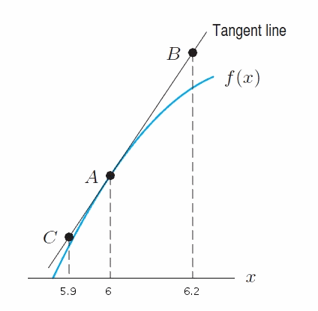
\includegraphics[width=0.5\linewidth]{2graph.png}
\end{center}
\begin{equation*}
A = \big( \hspace{0.5cm}, \hspace{0.5cm} ), \qquad B = \big( \hspace{0.5cm}, \hspace{0.5cm} ), \qquad C = \big( \hspace{0.5cm}, \hspace{0.5cm})
\end{equation*}
\end{problem}


\newpage

%%%%%%%%%%%%%%%%%%%%%%%%%%%%%%%%%%%%% Page 3
\noindent{\large\bf MATH 122}\hfill{\large\bf Exam \#2.}\hfill{\large\bf
  Fall 2016}\hfill{\large\bf Page 3/4}\hrule

\bigskip

\begin{problem}(7 pts each)
Find the derivative of the following functions:
\begin{enumerate}
\item $f(x) = \sqrt{\dfrac{1}{x^{39}}}$
\begin{flushright}
  \begin{tikzpicture}
    \draw (-4cm,0.5cm) node {$f'(x)=$};
    \draw (-3cm,-0.2cm) rectangle (5cm,1.2cm);
  \end{tikzpicture}
\end{flushright}
\item $y = 6t^5 - 10\sqrt{t} + \frac{9}{t}$
\begin{flushright}
  \begin{tikzpicture}
    \draw (-4cm,0.5cm) node {$y'(t)=$};
    \draw (-3cm,-0.2cm) rectangle (5cm,1.2cm);
  \end{tikzpicture}
\end{flushright}
\item $f(x) = (2^x + x^5)(3 - \ln x)$
\begin{flushright}
  \begin{tikzpicture}
    \draw (-4cm,0.5cm) node {$f'(x)=$};
    \draw (-3cm,-0.2cm) rectangle (5cm,1.2cm);
  \end{tikzpicture}
\end{flushright}
\item $f(x) = \dfrac{x^8+2}{x}$
\begin{flushright}
  \begin{tikzpicture}
    \draw (-4cm,0.5cm) node {$f'(x)=$};
    \draw (-3cm,-0.2cm) rectangle (5cm,1.2cm);
  \end{tikzpicture}
\end{flushright}
\item $f(x) = \ln \big(8 - e^{-x}\big)$
\begin{flushright}
  \begin{tikzpicture}
    \draw (-4cm,0.5cm) node {$f'(x)=$};
    \draw (-3cm,-0.2cm) rectangle (5cm,1.2cm);
  \end{tikzpicture}
\end{flushright}
\item $f(x) = \big( 6 + \ln x \big)^{0.6}$
\begin{flushright}
  \begin{tikzpicture}
    \draw (-4cm,0.5cm) node {$f'(x)=$};
    \draw (-3cm,-0.2cm) rectangle (5cm,1.2cm);
  \end{tikzpicture}
\end{flushright}
\item $f(x) = 2e^{7x} + e^{-x^6}$
\begin{flushright}
  \begin{tikzpicture}
    \draw (-4cm,0.5cm) node {$f'(x)=$};
    \draw (-3cm,-0.2cm) rectangle (5cm,1.2cm);
  \end{tikzpicture}
\end{flushright}
\end{enumerate}
\end{problem}

\newpage

%%%%%%%%%%%%%%%%%%%%%%%%%%%%%%%%%%%%% Page 4
\noindent{\large\bf MATH 122}\hfill{\large\bf Exam \#2.}\hfill{\large\bf
  Fall 2016}\hfill{\large\bf Page 4/4}\hrule

\bigskip

\begin{problem}[7 pts]
Find an equation for the tangent line to the graph of $f(x) = 3x^2-5x+6$ at $x=1$.

\vspace{4cm} 

\begin{flushright}
  \begin{tikzpicture}
    \draw (-3.5cm,0.5cm) node {$y=$};
    \draw (-3cm,-0.2cm) rectangle (5cm,1.2cm);
  \end{tikzpicture}
\end{flushright}
\end{problem}
\hrule

\begin{problem}[7 pts]
Find an equation for the tangent line to the graph of $f(x) = (2x^2-1)(3x+4)$ at $x=0$.

\vspace{5cm} 

\begin{flushright}
  \begin{tikzpicture}
    \draw (-3.5cm,0.5cm) node {$y=$};
    \draw (-3cm,-0.2cm) rectangle (5cm,1.2cm);
  \end{tikzpicture}
\end{flushright}
\end{problem}
\hrule

\begin{problem}[7pts]
The cost $C$ (in dollars) to produce $g$ gallons of a chemical can be expressed as $C = f(g)$.  Using units, explain the meaning of the following statements in terms of the chemical.
\begin{enumerate}
\item $f(400) = 500$.
\begin{flushright}
  \begin{tikzpicture}
    \draw (-8.5cm,0.5cm) node {The statement $f(400)=500$ means};
    \draw (-5cm,-0.2cm) rectangle (5cm,1.2cm);
  \end{tikzpicture}
\end{flushright}

\item $f'(400) = 6$
\begin{flushright}
  \begin{tikzpicture}
    \draw (-8.5cm,0.5cm) node {The statement $f'(400)=6$ means};
    \draw (-5cm,-0.2cm) rectangle (5cm,1.2cm);
  \end{tikzpicture}
\end{flushright}
\end{enumerate}
\end{problem}

\end{document}
